\section{PCE Maps - Choi matrix}
% 
\subsection{A single qubit}

We can write any quantum state associated to a qubit in the Bloch sphere parametrization as
% 
\begin{equation}
\rho=\frac{1}{2}\sum_{\alpha=0}^{3} r_{\alpha} \sigma_{\alpha}.
\label{rho2}
\end{equation}
% 
Moreover, it is possible to define a quantum map capable of modifying each of the coefficients $r_{\alpha}$, these are known as \textit{Pauli maps}
% 
\begin{equation}
\rho \to \rho'=\mathcal{E}[\rho ]=\frac{1}{2}\sum_{\alpha=0}^{3} \tau_{\alpha} r_{\alpha} \sigma_{\alpha},
\label{Pauli_Map}
\end{equation}
% 
with $-1\leq \tau_{\alpha} \leq 1$. 

We now turn to find the matrix form of the map $\mathcal{E}$ in order to construct the Choi matrix and the conditions the set of parameters $\{\tau_{\alpha}\}$ need to satisfy in order to $\mathcal{E}$ be considered a quantum channel. By writing the density matrix in vector form $\kket{\rho}=2^{-1}\sum_{\alpha=0}^{3} r_{\alpha} \kket{\sigma_{\alpha}}$, the matrix form of the map $\mathcal{E}$ may be written as
% 
\begin{equation}
\hat{\mathcal{E}} = \frac{1}{2}\sum_{\alpha=0}^{3} \tau_{\alpha} \ddyada{\sigma_{\alpha}},
% \label{Map_Pauli}
\end{equation}
%
where the kets $\kket{\sigma_{\alpha}}$ correspond to the vectorized elements of the Pauli basis and satisfy the usual relation $ \bbrakket{{\sigma_{\alpha}}}{{\sigma_{\alpha'}}} = \tr \left(\sigma_{\alpha}^{\dagger} \sigma_{\alpha'}\right) = 2 ~\delta_{\alpha\alpha'}$. After some steps it is possible to show that the associated Choi matrix reads
% 
\begin{equation}
 \mathcal{D} = \frac{1}{2}\sum_{\alpha=0}^{3} \tau_{\alpha} \sigma_{\alpha} \otimes \sigma_{\alpha}^*.
%  \label{Choi_1}
\end{equation}
% 
Moreover, observe that $\mathcal{D}$ has the same form as the matrix representation of a random unitary channel, with Kraus operators given by $K_{\alpha}=\sqrt{\tau_{\alpha}/2}\sigma_{\alpha}$ \cite{CHRUSCINSKI20131425}. In this way the Choi matrix $\mathcal{D}$ is diagonal in the Pauli basis (see Appendix for details),
%
\begin{equation}
 \mathcal{D} \kket{\sigma_{\alpha}}= \lambda_{\alpha} \kket{\sigma_{\alpha}},
\end{equation}
% 
with eigenvalues given by 
% 
\begin{equation}
 \lambda_{\alpha} = \sum_{\beta=0}^3\sa_{\alpha\beta}\tau_{\beta},
\end{equation}
%
or more compactly $\vec{\lambda} = \sa~\vec{\tau}$, where $\sa=2^{-1}H\otimes H$ and $H$ is the Hadamard matrix,
%
\begin{equation}
 H=\begin{pmatrix}
        1 & 1\\
        1 & -1\\
    \end{pmatrix}.
 \label{Hadd_Mat}
\end{equation}
% 

\subsection{$N$ qubits}
% 
For the case of $N$ qubits, the density matrix may be written as
% 
\begin{equation}
\rho=\frac{1}{2^N}\sum_{\vec{\alpha}} r_{\vec{\alpha}} \sigma_{\vec{\alpha}}.
% \label{rho2}
\end{equation}
% 
Analogously to the single qubit case, one can define the $N$-qubits Pauli map $\mathcal{E}_N$
% 
\begin{equation}
\rho \to \rho'=\mathcal{E}_N[\rho ]=\frac{1}{2^N}\sum_{\vec{\alpha}} \tau_{\vec{\alpha}} r_{\vec{\alpha}} \sigma_{\vec{\alpha}},
% \label{Pauli_Map}
\end{equation}
% 
with $-1\leq \tau_{\vec{\alpha}} \leq 1$. 
% 
In this case the density matrix in vector form holds 
% 
\begin{equation}
 \kket{\rho}=\frac{1}{2^N}\sum_{\vec{\alpha}} r_{\vec{\alpha}} \kket{\sigma_{\vec{\alpha}}},
\end{equation}
% 
where $\kket{\sigma_{\vec{\alpha}}}=\kket{\sigma_{\alpha_1}}\otimes\dots \otimes\kket{\sigma_{\alpha_N}}$, and satisfy the usual orthogonality relation $\bbrakket{{\sigma_{\vec{\alpha}}}}{{\sigma_{\vec{\alpha}'}}} = \tr \left(\sigma_{\vec{\alpha}}^{\dagger} \sigma_{\vec{\alpha}'}\right) = 2^N ~\delta_{\vec{\alpha}\vec{\alpha}'}$. The matrix representation of this map is given by
% 
\begin{equation}
\hat{\mathcal{E}}_N = \frac{1}{2^N}\sum_{\vec{\alpha}} \tau_{\vec{\alpha}} \ddyada{\sigma_{\vec{\alpha}}}.
% \label{Map_Pauli}
\end{equation}
%
As in the previous case, the Choi matrix $\mathcal{D}_N$ may be written in terms of tensor products of Pauli matrices
% 
\begin{equation}
 \mathcal{D}_N = \frac{1}{2^N}\sum_{\vec{\alpha}} \tau_{\vec{\alpha}}  \bigotimes_{j=1}^N \sigma_{\alpha_j} \otimes \sigma_{\alpha_j}^*.
%  \label{Choi_1}
\end{equation}
% 
After several steps, it is possible to prove that analogously to the single qubit case, $\mathcal{D}_N$ is diagonal in the $N$-qubits Pauli basis
%
\begin{equation}
 \mathcal{D}_N \kket{\sigma_{\vec{\alpha}}}= \lambda_{\vec{\alpha}} \kket{\sigma_{\vec{\alpha}}},
\end{equation}
% 
with eigenvalues $\lambda_{\vec{\alpha}}$ given by 
% 
\begin{equation}
 \lambda_{\vec{\alpha}} = \sum_{\vec{\beta}} \san_{\vec{\alpha}\vec{\beta}}\tau_{\vec{\beta}},
\end{equation}
%
where 
% 
\begin{equation}
 \san=\sa^{\otimes N}=\frac{1}{2^N}\left(H\otimes H\right)^{\otimes N}=\left(\frac{H}{\sqrt{2}}\right)^{\otimes 2N}.
\end{equation}
%

\section{Bloch-like parametrization for a single qudit}
% 
One of the ways we can generalize the Bloch parametrization for individual high dimensional quantum systems (or qudits), is to employ the so called \textit{Weyl basis} \cite{Bertlmann2008}. Under this parametrization any density matrix $\rho$ may be written as
% 
\begin{equation}
\rho=\sum_{mn=0}^{d-1} \alpha_{mn} U_{mn},
\label{rho}
\end{equation}
% 
where $U_{mn}$ are the Weyl operators, given by
% 
\begin{equation}
U_{mn}=\sum_{j=0}^{d-1}\omega_d^{j m}\dyad{j}{j\oplus n},
\label{Umn}
\end{equation}
% 
and $\omega_d=\exp(2\pi i/d)$ is the primitive $d$-th root of unity. Note that for the case of qubits ($d=2$), the set $\{U_{mn}\}$ reduces to the Pauli matrices and the identity (see Fig. \ref{Weyl_Pauli}).

\begin{figure}[h]
  \centering
  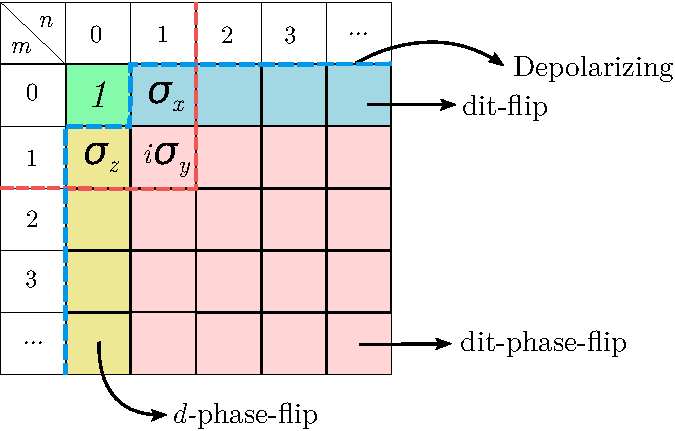
\includegraphics[scale=0.65]{Weyl_2.pdf}
  \caption{Relation between Weyl operators and Pauli matrices. Note that the Weyl operators may also be employed to generalize some usual unital channels. Taken from \cite{Fonseca2019}.}
  \label{Weyl_Pauli}
\end{figure}
% 
Due to the fact that the Weyl operators are not Hermitian, then the coefficients $\alpha_{mn}$ are in general complex.

\section{Weyl maps}

Consider the generalization of the Pauli maps for qudits as
% 
\begin{equation}
\rho \to \rho'=\mathcal{E}[\rho ]=\sum_{m,n=0}^{d-1} \tau_{mn} \alpha_{mn} U_{mn},
\label{Weyl_Map}
\end{equation}
% 
with $-1\leq \tau_{mn} \leq 1$. 

Our task is now to find the associated matrix form. For this let write $\rho$ in vector form
% 
\begin{equation}
\ket{\rho} = \sum_{m,n=0}^{d-1} \alpha_{mn} \ket{U_{mn}},
% \label{Weyl_Map}
\end{equation}
% 
with
% 
\begin{equation}
\ket{U_{mn}}=\sum_{j=0}^{d-1}\omega_d^{j m}\ket{j,j\oplus n}.
\label{Ket_U}
\end{equation}
% 
From this, it can be easily seen that the matrix form of the map in Eq. \ref{Weyl_Map} can be written as
% 
\begin{equation}
\hat{\mathcal{E}} = \frac{1}{d}\sum_{m,n=0}^{d-1} \tau_{mn} \dyad{U_{mn}},
\label{Map_Pauli}
\end{equation}
% 
where we have used the fact that
% 
\begin{equation}
 \tr \left(U_{mn}^{\dagger} U_{kl}\right) = \braket{{U_{mn}}}{{U_{kl}}} = d ~\delta_{mk}\delta_{nl}.
\end{equation}
% 
By substituting Eq. \ref{Ket_U} in Eq. \ref{Map_Pauli}, we obtain the matrix form of the map in the computational basis
% 
\begin{equation}
 \hat{\mathcal{E}}_c = \frac{1}{d}\sum_{jk\mu\nu=0}^{d-1} \tau_{\mu\nu}~ \omega_d^{\mu (j-k)} \dyad{j,j\oplus \nu}{k,k\oplus \nu}.
\end{equation}
% 
Applying the reshuffling operation and after some steps it is possible to see that the Choi matrix reads
% 
\begin{align}
 \mathcal{D} &=  \frac{1}{d}\sum_{jk\mu\nu=0}^{d-1} \tau_{\mu\nu}~ \omega_d^{\mu (j-k)} \dyad{j,k}{j\oplus \nu,k\oplus \nu},\\
 & = \frac{1}{d}\sum_{\mu\nu=0}^{d-1} \tau_{\mu\nu} ~U_{\mu\nu}\otimes U_{\mu\nu}^*.
 \label{Choi_1}
\end{align}
% 
This expression is valid for arbitrary $d$ and may provide some hints into the search of a simpler form for the proof of the diagonalization of $\mathcal{D}$. In particular, for $d=2$ we have
%  
\begin{equation}
  \mathcal{D} = \frac{1}{2}\sum_{\mu=0}^{3} \tau_{\mu} ~\sigma_{\mu}\otimes \sigma_{\mu}^*,
\end{equation}
% 
note that in the last expression we have used one index instead of two binary ones.

\section{Diagonalization of the Choi Matrix}
% 
\subsection{Numerical approach on WCE maps}
% 
We carried out a first (non exhaustive) numerical approach in which we considered $\tau$ coefficients either equal to zero or one, for the case of a qutrit ($d=3$). In Table \ref{Table1}, we list the set of trace preserving channels found so far (however, by symmetry reasons I am almost sure there are no more channels).
% 
\begin{table}[h]
 \centering
\begin{tabular}{ |c|c|c|c|c|c| } 
\hline
$\tau$ & $D$ & $t_1$ &$t_2$ &$t_3$ & $I$\\
\hline
$\tau_{00}$ & 1 & 1 & 1 & 1& 1\\ 
\hline
$\tau_{01}$ &  & 1 & && 1\\ 
\hline
$\tau_{02}$ & & 1 & && 1\\ 
\hline
$\tau_{10}$ & &  & 1 & & 1\\ 
\hline
$\tau_{11}$ &  &  & & 1& 1\\ 
\hline
$\tau_{12}$ &  &  & && 1\\ 
\hline
$\tau_{20}$ &  &  & 1&& 1\\ 
\hline
$\tau_{21}$ &  &  & && 1\\ 
\hline
$\tau_{22}$ &  &  & & 1& 1\\ 
\hline
\end{tabular}
\caption{List of ``Weyl component erasing'' (WCE) channels for a single qutrit. Each column shows the non-null coefficients $(\tau_{mn}=1)$ leading to real non-negative eigenvalues of the Choi matrix $\mathcal{D}$.}
\label{Table1}
\end{table}
% 

In summary, we have 5 WCE channels on qutrits:
\begin{itemize}
 \item 1 completely depolarizing channel ($D$).
 \item 3 three components channels ($t_j$).
 \item 1 Identity channel ($I$).
\end{itemize}

\subsection{Analytical derivation }
% 
Recalling Eq. \ref{Choi_1}, we can write the Choi matrix associated to a Weyl channel as
% 
\begin{equation}
 \mathcal{D} =  \frac{1}{d}\sum_{jk\mu\nu=0}^{d-1} \tau_{\mu\nu}~ \omega_d^{\mu (j-k)} \dyad{j,k}{j\oplus \nu,k\oplus \nu}.
\end{equation}
% 
After some steps we obtain 
% 
\begin{equation}
 \mathcal{D} =  \frac{1}{d}\sum_{kl=0}^{d-1} \left(\frac{1}{d}\sum_{\mu\nu=0}^{d-1}\tau_{\mu,\nu}~ \omega_d^{k\nu -\mu l} \right)\dyad{U_{kl}}.
\end{equation}
% 
In this way, the basis with elements $d^{-1/2}\ket{U_{kl}}$ diagonalizes the Choi matrix, and the corresponding eigenvalues read
% 
\begin{equation}
 \lambda_{kl}=\frac{1}{d}\sum_{\mu\nu=0}^{d-1}\tau_{\mu\nu}~ \omega_d^{k\nu -\mu l}.
\end{equation}
% 
Note that we recover the previous results for $d=2$, as expected. In addition, we can rewrite the above expression in vector form as
% 
\begin{equation}
 \vec{\lambda}=F\otimes F^*~\vec{\tau},
\end{equation}
% 
where $F$ is the matrix associated to a quantum Fourier transform
% 
\begin{equation}
 F=\frac{1}{\sqrt{d}}\sum_{k,l=0}^{d-1}\omega_d^{kl}\dyad{k}{l}.
\end{equation}
% 
Finally, I am almost sure that the results from the previous subsection may be obtained using the fact that $\sum_k\omega_d^{k(m-n)}=d~\delta_{mn}$.

\section{Generalization to $N$ qudits}
% 
In analogy to the problem of two level systems, the generalization to the case of arbitrary number of qudits is relatively straightforward. Work in progress...
